\documentclass{article}

% CS230 project report template, built on the official NeurIPS 2026 style file.
% Keep the [final] option: it prints the author block and omits line numbers.
% natbib is loaded by the style file; this makes citations numeric, e.g. [1, 2].
\PassOptionsToPackage{numbers,compress}{natbib}
\usepackage[final]{neurips_2026}

\usepackage[utf8]{inputenc} % allow utf-8 input
\usepackage[T1]{fontenc}    % use 8-bit T1 fonts
\usepackage{hyperref}       % hyperlinks
\usepackage{url}            % simple URL typesetting
\usepackage{booktabs}       % professional-quality tables
\usepackage{amsfonts}       % blackboard math symbols
\usepackage{amsmath}        % \operatorname
\usepackage{nicefrac}       % compact symbols for 1/2, etc.
\usepackage{microtype}      % microtypography
\usepackage{xcolor}         % colors
\usepackage{graphicx}       % figures
% Page limit for the main content, used in the text below. Update it here only.
\newcommand{\pagelimit}{5}

% LENGTH (course rule): at most \pagelimit{} pages, excluding references, contributions, AI disclosure and the
% appendix; TAs may not read the appendix. The outline budgets add up to about 2,100 words of prose next to the
% 6 floats of the main text (figures 1--3, tables 1--3).
% DRAFTING AIDS (none left in the text since 2026-11-19; the macros stay defined, unused):
%   \outline{...}  blue: Claude's outline of the facts a section needs. Replace it with your own prose.
%   \tbd{...}      red: a number or item still to come (test numbers arrive with the Step 8 test run).
\newcommand{\outline}[1]{{\color{blue!55!black}\small #1}}
\newcommand{\tbd}[1]{{\color{red}[#1]}}

\title{Skier Tracking and 2D Body-and-Ski Landmark Estimation}

\author{%
  Ruichao Zhang \\
  \texttt{ruichaoz@stanford.edu} \\
}

\begin{document}

\makeatletter\global\@topnum\z@\makeatother % no floats above the title, as article.cls does
\maketitle

\begin{abstract}
% Ruichao's text (2026-11-18), proofread; the optional clause on the perception layer added, as agreed.
Reviewing ski runs on video is difficult, motivating automatic technique feedback; we build the tracking and landmark
layer it needs. COCO-trained pose models omit ski landmarks, and generic trackers drift on broadcast footage. We
combine a fixed SiamFC tracker, a COCO-pretrained HRNet-W32 fine-tuned to 24 body, ski and pole landmarks, a
pose-guided second pass on the same frame, and a smoothed, skier-centered replay. A rule fixed in advance selects
crop jitter from an augmentation study. Test ski accuracy (percentage of correct keypoints, PCK@0.1) reaches 94.8\% on
well-framed crops but 81.2\% on events absent from training. Tracker crops cost 28.0 ski points; refinement recovers
9.3 without labels or retraining. Crop jitter shows no clear gain on well-framed test crops but adds 1.6 points on
tracker crops and 4.6 on follow-camera footage. The replay keeps 93.7\% of ski ends visible, short of its 95\% target.
After the test freeze, off-the-shelf STARK raises tracker-crop ski accuracy from 67.7\% to 86.5\%, supporting tracking
as the main bottleneck, and pseudo-labels raise the other-event score to 89.3\%.
\end{abstract}

\section{Introduction}
% Ruichao's text (2026-11-18), proofread; the three optional additions applied, as agreed.
Reviewing a ski run on video is difficult: broadcast cameras pan and zoom, the skier is small and often obscured by
gates, and thin, fast-moving skis overlap. Our long-term goal is automatic technique feedback, but the datasets lack
expert technique annotations, so we build the tracking and landmark layer such feedback requires. COCO-trained pose
models predict no ski landmarks, while generic trackers drift on broadcast skiing, as
the SkiTB skier-tracking benchmark shows; better tracking also improves pose estimation~\cite{dunnhofer2024tracking}.

Our input is a single-camera skiing video and a box around the skier in its first frame. The pipeline
(Figure~\ref{fig:pipeline}) combines a fixed tracker, a crop, a fine-tuned HRNet-W32 CNN, and a pose-guided second
pass, and outputs 24 2D landmarks per frame (14 body, 8 ski, 2 pole) and a smooth, skier-centered 16:9 replay with a
skeleton overlay.

We contribute a controlled, tracker-aware augmentation study (crop jitter, blur, occlusion) with paired seeds and a
selection rule fixed in advance; a simple same-frame pose-guided re-crop without labels or retraining; and paired
measurements of tracking's pose-accuracy cost across tracker-overlap levels. This project is not shared with another
class.

\begin{figure}[hb]
  \centering
  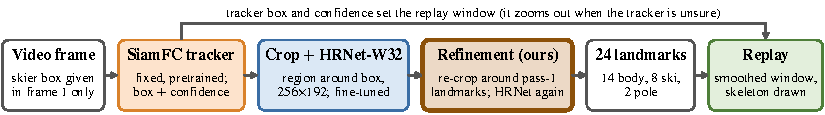
\includegraphics[width=\linewidth]{figures/pipeline.pdf}
  \caption{The system, per video frame. Only the pose model is trained; refinement runs it twice.}
  \label{fig:pipeline}
\end{figure}

\section{Related work}
% Ruichao's text (2026-11-18), proofread; all 12 Related work citations verified (references.bib header).
Ski 2DPose~\cite{bachmann2019motion} provides 24 body, ski and pole landmarks on broadcast footage, built for 3D
motion capture from pan-tilt cameras. SkiTB~\cite{dunnhofer2024tracking}, a skier-tracking benchmark, fine-tunes
AlphaPose~\cite{fang2023alphapose} on Ski 2DPose and links tracking quality to pose accuracy; its PCK uses half the head--neck length,
preventing direct comparison with our scores. SkiTechCoach~\cite{hirano2025skitechcoach} pairs simulator 3D poses
and sole pressure with expert coaching feedback; we build perception for such feedback on broadcast video.

HRNet~\cite{sun2019deep} repeatedly fuses high- and low-resolution branches, while Simple
Baselines~\cite{xiao2018simple} uses deconvolution layers on a ResNet backbone; both depend on well-framed person
crops. We adapt MMPose's COCO-pretrained HRNet-W32~\cite{mmpose2020}, extending beyond COCO's 17 body-only
keypoints~\cite{lin2014microsoft}.

SiamFC~\cite{bertinetto2016fully} cross-correlates a first-frame template with search regions. We use the released
siamfc-pytorch weights~\cite{huang2019siamfcpytorch}, whose training script uses GOT-10k~\cite{huang2019got}.
STARK~\cite{yan2021learning} combines transformer-based box prediction with template updates.

Xiao et al.~\cite{xiao2018simple} propagate joints through optical flow and build next-frame boxes around them,
enlarged by 15\%; our refinement instead re-crops the same frame from its own first-pass landmarks. Noisy
Student~\cite{xie2020self} iteratively trains larger, noised models on labeled and teacher-pseudo-labeled data; our
lite pose variant uses one round and filters labels by agreement between two teachers.

\section{Dataset}
% Ruichao's text (2026-11-16), proofread; the per-video accuracies moved to Section 5.2.
Ski 2DPose~\cite{bachmann2019motion} contains 1,982 images from 16 alpine YouTube videos (Creative Commons),
sparsely annotated across 158 single-camera segments with 24 visibility-flagged landmarks (14 body, 8 ski, 2 pole).
To prevent near-duplicate leakage, we split by video: train/val/test contain 4/3/3 videos and 1,194/293/360 images.
Six follow-cam videos (134 images), filmed by a camera following the skier on training runs, provide a separate
out-of-distribution evaluation, performed once. One record without a reference box is excluded. All four training videos come from the Almaty 2017 Universiade; validation uses Trentino
2013 and Granada 2015. The Almaty giant-slalom test video contributes 80\% of the test ski labels (accuracy by event:
Section~\ref{sec:pose_alone}).

SkiTB~\cite{dunnhofer2024tracking} (CC BY-NC 4.0) provides boxes without landmarks for 100 alpine sequences, with an
official athlete train/val/test split of 53/6/41. Tracking uses single-camera clips: 75 validation and 471 test
clips. For pose crops, reference
boxes tightly enclose the visible body and ski labels, are expanded $1.25\times$ and fitted to 3:4; crops are warped
to $256\times192$. Targets are $64\times48$ Gaussian heatmaps ($\sigma=2$\,px). Standard augmentation uses horizontal
flips ($p=0.5$; left/right labels swapped), $\pm15^\circ$ rotation, and 0.8--1.2 scaling.

\section{Methods}
% Ruichao's text (2026-11-16), proofread; trims (i)-(v) applied; 3 paragraphs and an inline refinement formula to save
% space. The loss matches skier.pose.loss.masked_mse.
The top-down HRNet-W32 (Figure~\ref{fig:hrnet}) processes one person per crop. We initialize its
28.5M-parameter backbone
from MMPose's COCO checkpoint~\cite{mmpose2020,sun2019deep}, replacing the $1\times1$, 32$\to$17 output layer with a
randomly initialized 32$\to$24 head (792 parameters). We minimize the masked heatmap MSE
\[
  \mathcal{L} = \frac{\sum_{i,j} v_{ij}\,\operatorname{mean}_{u,v}\big(\hat H_{ij}(u,v) - H_{ij}(u,v)\big)^2}
                     {\max\big(1, \sum_{i,j} v_{ij}\big)},
\]
where $\hat H_{ij}$ and $H_{ij}$ are the predicted and target heatmaps of joint $j$ in sample $i$, and $v_{ij}=1$ for
visible labels inside the crop, otherwise zero (no gradient).

\begin{figure}[h]
  \centering
  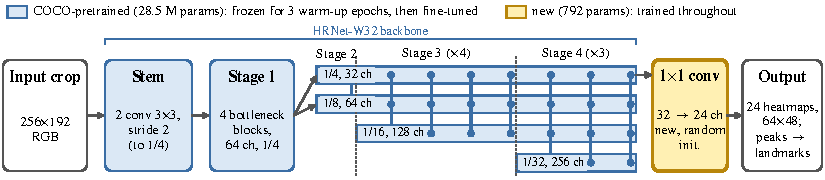
\includegraphics[width=\linewidth]{figures/hrnet.pdf}
  \caption{The pose model. HRNet-W32~\cite{sun2019deep} keeps a 1/4-resolution branch throughout and adds
  lower-resolution branches that exchange information after every module (vertical lines). Its COCO weights (blue)
  stay frozen for 3 warm-up epochs while the new 24-landmark output layer (yellow) learns; then the whole network is
  fine-tuned.}
  \label{fig:hrnet}
\end{figure}

We train with Adam~\cite{kingma2015adam} and batches of 16. Three warm-up epochs train only the head (learning rate
$10^{-3}$), freezing backbone weights and BatchNorm statistics. Whole-network training then runs for 150 epochs
(backbone $10^{-4}$, head $5\times10^{-4}$), reducing the rates tenfold at epochs 90 and 127. We retain the checkpoint
with the best validation ski PCK; each of the two seeds uses the same data order for every
recipe. E1 uses standard augmentation. Relative to E1, E2 adds tracker-like crop jitter (center $\pm10\%$ per axis;
size $\times$0.9--1.1); E3 adds motion blur ($p=0.5$, 3--9\,px) and an occluding patch ($p=0.5$, 5--15\% of the
crop); E4 adds all three.

SiamFC (released siamfc-pytorch weights~\cite{bertinetto2016fully,huang2019siamfcpytorch}) is initialized once per
clip from its first-frame box. Confidence is the peak of its sum-normalized response map; Youden's
$J$~\cite{youden1950index} on the SkiTB validation clips sets the threshold (failure: IoU $<0.1$).
The tracker box is expanded before standard padding. Our geometric refinement constructs $B =
k_{\mathrm{ref}}\cdot\operatorname{tight}\{\hat x_j : j \in \text{body}\cup\text{ski},\ s_j \ge s_{\min}\}$ from
pass-1 predictions $\hat x_j$ and scores $s_j$, applies training preprocessing, and reruns the same model. With fewer
than four qualifying points, pass 1 is kept. Replay exponentially smooths an enlarged 16:9 tracker window with a
minimum size; low-confidence frames hold its center and zoom out.

\section{Experiments and Results}
\subsection{Setup}
\label{sec:setup}
% Ruichao's text (2026-11-16), proofread.
All settings were chosen without test data by rules fixed before each run, except the replay smoothing and width,
which we set by judgment from the validation trade-off (appendix Table~\ref{tab:choices}). After
recording split, configuration and checkpoint hashes, the main test evaluation ran once (2026-11-12, commit
\texttt{bf546e3}). The choices were 150
fine-tune epochs (ski tails unlearned at 50), recipe E2, crop expansion $\times1.1$
before the $\times1.25$ padding, raw SiamFC confidence (AUC 0.83; 0.63 when divided by its median over the first 10
tracked frames), replay $\tau=0.2$\,s and width $2.5\times$ the tracker box, and refinement
$s_{\min}=0.3$, $k_{\mathrm{ref}}=1.3$ (grids: appendix Table~\ref{tab:grids_val}).

PCK@$t$ is the share of visible landmarks predicted within $t$ times the diagonal of the tight box around the labeled
body and ski points ($t=0.1$, $0.05$); body and ski are reported separately, poles as a supplement. Tracking uses IoU,
success AUC, and the SkiTB toolkit's F-score. Replay uses the share of the SkiTB ground-truth box inside the replay
window, the share of visible Ski 2DPose ski-end labels inside it (target, set in advance: at least 95\%), and the mean
acceleration of the window center (frame diagonals/s$^2$). Brackets give 95\%
cluster-bootstrap intervals~\cite{efron1994introduction} (10,000 resamples; segments within videos for pose, SkiTB
sequences for tracking); differences are computed before rounding. Pose baselines are E0 (the COCO model, on 10 shared body
landmarks) and E1 (plain fine-tuning). Pose accuracy under tracking needs landmark labels, so it is measured on the
Ski 2DPose videos: the tracker starts from the reference box at each segment's first labeled frame, and subsequent labeled
frames are scored against the same labels using reference (label-dependent upper bound), tracker (baseline), and
refined crops (Table~\ref{tab:system}; Figure~\ref{fig:strata}).

\subsection{Pose model alone: the augmentation study}
\label{sec:pose_alone}
% Ruichao's text (2026-11-16), proofread. The follow-cam viewpoint facts moved to the Analysis outline.
Table~\ref{tab:pose}'s validation results select E2 under the rule fixed in advance: ski PCK@0.1 is 93.1\%, versus
91.9/92.0/91.0\% for E1/E3/E4, with no recipe losing body accuracy. E2 $-$ E1 is $+1.2$ points [0.1, 2.3], rising to
$+2.5$ [1.5, 3.6] under moderate crop error. E3/E4 improve body accuracy ($+1.7$/$+1.9$) but not ski accuracy (appendix Table~\ref{tab:aug_val}).

On the test set, evaluated once, E1 beats E0 (which predicts no skis) on the 10 shared body landmarks only at the
stricter PCK@0.05 ($+4.9$ [2.6, 7.0]; PCK@0.1: $+1.5$ [$-1.0$, 3.7]). E2 $-$ E1
shows no clear ski or body difference at PCK@0.1 (Table~\ref{tab:pose}) but gains $+1.2$ [0.2, 2.2] at ski PCK@0.05.

However, 80\% of the test ski labels come from the training-event video: E2 scores 98.1\% there versus 81.2\% on the
other two videos (appendix Table~\ref{tab:extras}(b)). Thus the
overall 94.8\% $\approx 0.8\times98.1 + 0.2\times81.2$, and the validation-to-test rise is confounded by event
composition. Post hoc, E2 $-$ E1 is $+1.4$ [0.8, 2.1] on the training event but $-2.3$ [$-6.4$, 0.9] on the
other-event videos (76 images; appendix Table~\ref{tab:cross_event}).

On follow-cam, ski accuracy falls to 73.5\%/78.1\% for E1/E2 (E2 $-$ E1: $+4.6$ [2.9,
6.7] over six videos); body stays at 97.4/97.5\%. Crop jitter helps on follow-cam; gains across events
remain uncertain.

\begin{table}[h]
  \centering
  \small
  \setlength{\tabcolsep}{3.5pt}
  \begin{tabular}{lcc|ccc|c}
    \toprule
    & \multicolumn{2}{c|}{Val (chose the recipe)} & \multicolumn{3}{c|}{Test (once)} & Follow-cam \\
    Run & Ski @0.1 & Ski, crop error$^{\dagger}$ & Body @0.1 & Ski @0.1 & Ski @0.05 & Ski @0.1 \\
    \midrule
    E0 COCO, not fine-tuned & -- & -- & 94.7$^{*}$ & -- & -- & -- \\
    E1 standard aug. & 91.9 & 90.4 & 96.3 & 94.1 & 89.8 & 73.5 \\
    E2 + crop jitter & \textbf{93.1} & \textbf{92.9} & 95.9 & 94.8 & 91.0 & 78.1 \\
    E3 + blur, occlusion & 92.0 & 90.9 & -- & -- & -- & -- \\
    E4 all three & 91.0 & 89.5 & -- & -- & -- & -- \\
    \midrule
    E2 $-$ E1 & $+1.2$ & $+2.5$ & $-0.5$ & $+0.7$ & $+1.2$ & $+4.6$ \\
    {\scriptsize 95\% CI} & {\scriptsize $[0.1, 2.3]$} & {\scriptsize $[1.5, 3.6]$} & {\scriptsize $[-1.3, 0.2]$}
      & {\scriptsize $[-0.3, 1.5]$} & {\scriptsize $[0.2, 2.2]$} & {\scriptsize $[2.9, 6.7]$} \\
    \bottomrule
  \end{tabular}
  \caption{The augmentation study, PCK (\%), two seeds pooled, reference crops (val/test/follow-cam: 293/360/134
  images). The rule fixed in advance (highest val ski @0.1, at most 2 points of body loss) picked E2; only E1 and E2
  went to test and follow-cam. $^{\dagger}$Boxes shifted by 10\% and rescaled by up to $1.1\times$. $^{*}$10 shared
  COCO landmarks (E1: 96.2, E2: 95.6). Differences are computed before rounding.}
  \label{tab:pose}
\end{table}

\subsection{Integrated system}
\label{sec:system}
% Ruichao's text (2026-11-18), proofread; the tracker paragraph moved first and "(smoother)" added, as agreed.
On 471 SkiTB test clips, SiamFC achieves mean IoU 0.404 [0.380, 0.428] and toolkit F-score 0.406, with
258 failure episodes (IoU $<0.1$ for $\ge0.5$\,s) across 234 clips. On the same clips, replay box containment is
0.963 [0.951, 0.973], and acceleration falls from 4.11 unsmoothed to 1.38 (3.0-fold smoother). On the
Ski 2DPose test segments, ski-end containment reaches 93.7\% (974/1,040) [86.5, 99.4], missing the 95\% target
(validation: 99.4\%).

Relative to the label-dependent reference upper bound, tracker crops cost E2 18.1 body and 28.0 ski points at
PCK@0.1 on test (Table~\ref{tab:system}; ski: 95.7$\to$67.7, interval [19.3, 37.7]), versus 14.8/18.4 on validation (appendix
Table~\ref{tab:system_val}).
Refinement adds $+9.3$ ski [6.7, 12.1] and $+3.5$ body [1.3, 6.0] points, recovering 33\% of the ski cost
(validation: 32\%) and 19\% of the body cost. Ski labels outside the crop fall from 30.5\% to 19.9\%; refinement falls back to pass 1 on 8--10\% of frames.

Figure~\ref{fig:strata} shows the largest recovery under partial overlap (IoU 0.1--0.5: ski 68.6$\to$84.4), with
smaller gains at IoU $\ge0.5$ (90.5$\to$94.9). At IoU $<0.1$, accuracy rises from 6.7\% to only 14.3\%, far below the
98.4\% reference result: refinement cannot rescue a lost tracker. Crop jitter helps under tracking: E2 exceeds E1 by
1.6 ski points [0.8, 2.5] on tracker crops and 1.9 [1.0, 2.8] after refinement.

\begin{table}[h]
  \centering
  \small
  \setlength{\tabcolsep}{4pt}
  \begin{tabular}{lcccc}
    \toprule
    Crop & E1 body & E1 ski & E2 body & E2 ski \\
    \midrule
    Reference (upper bound) & 97.1 & 94.5 & 97.1 & 95.7 \\
    Tracker (baseline) & 79.0 & 66.1 & 78.9 & 67.7 \\
    Refined (ours) & 82.1 & 75.1 & 82.4 & 77.0 \\
    \midrule
    Refined $-$ tracker & $+3.0$ $[0.9, 5.6]$ & $+9.0$ $[6.4, 11.9]$ & $+3.5$ $[1.3, 6.0]$ & $+9.3$ $[6.7, 12.1]$ \\
    \bottomrule
  \end{tabular}
  \caption{Pose under tracking on test, PCK@0.1 (\%) on the same 317 labeled frames (40 segments), seeds pooled.
  Reference crops need the labels; last row: gain over the tracker crop, 95\% CI. Differences are computed before
  rounding.}
  \label{tab:system}
\end{table}

\begin{figure}[h]
  \centering
  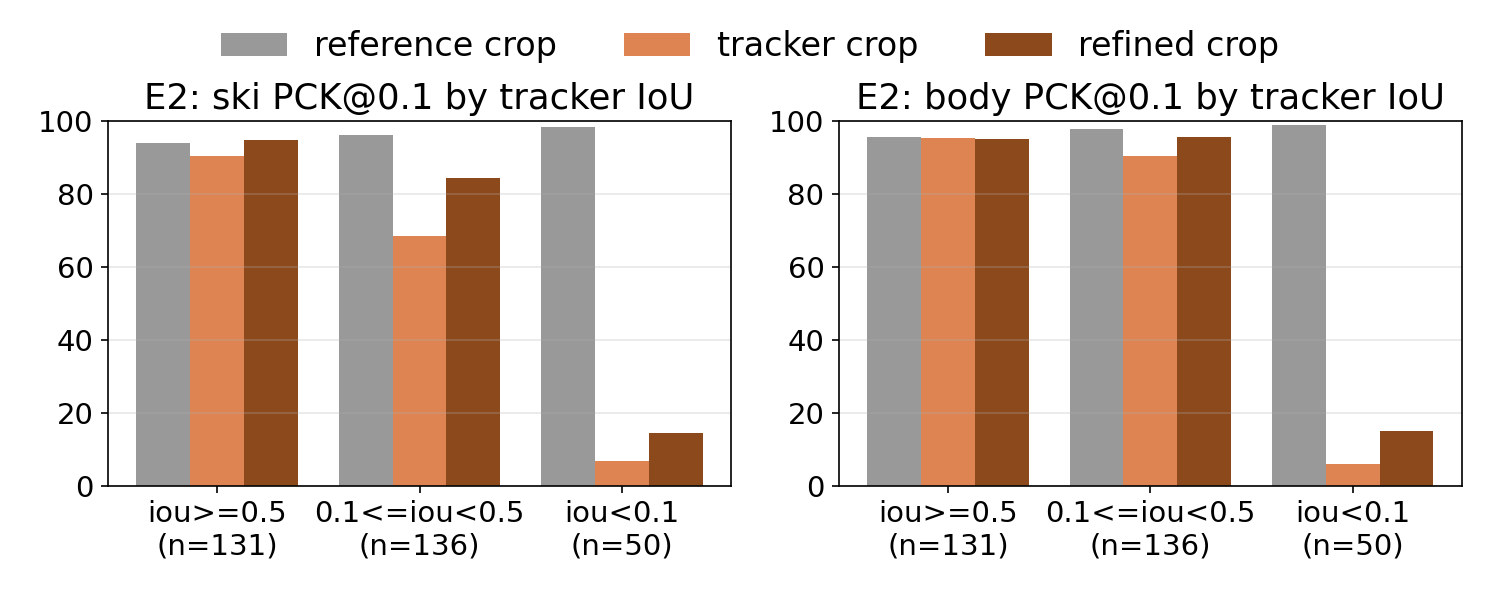
\includegraphics[width=0.5\linewidth]{figures/propagation_strata_test.png}
  \caption{E2 pose accuracy from reference (gray), tracker (orange) and refined (brown) crops on test, by IoU between
  tracker and reference box; $n$: labeled frames per bin.}
  \label{fig:strata}
\end{figure}

\subsection{Extra experiments after the test freeze: a stronger tracker and pseudo-labels}
\label{sec:extra}\label{sec:extra_pl}
% Ruichao's text (2026-11-18), proofread; optional addition 1 (the filter's validation precision) added, as agreed.
% The per-joint ski-tail facts moved to the Analysis outline.
Both experiments were decided after the main test result, fixed on validation and tested once; they leave
Tables~\ref{tab:pose}--\ref{tab:system} unchanged (details: appendix Table~\ref{tab:extras}).

Off-the-shelf STARK-ST50~\cite{yan2021learning} replaces SiamFC without fine-tuning on skiing; only its confidence
threshold is recalibrated by the same rule. SkiTB IoU rises from 0.404 to 0.679, tracker-crop ski from 67.7 to 86.5
($+18.8$ [11.1, 27.8]) and refined ski from 77.0 to 92.1; failure episodes fall from 258 to 66 (appendix
Figure~\ref{fig:stark_success}). Its toolkit F-score, 0.677, is close to SkiTB's reported
0.671~\cite{dunnhofer2024tracking}. Refinement still adds 5.6 ski points [2.7, 9.0], and the replay keeps 99.8\% of ski
ends in view, at higher acceleration (1.38$\to$1.69).

The pseudo-label student (PL) trains on real images plus SkiTB training frames labeled by E2, a lite form of Noisy
Student~\cite{xie2020self} (one round, about 10\% of eligible frames). A filter chosen on validation keeps only
joints that both teachers score confidently and agree on: over 95\% correct at PCK@0.05, versus 84--89\% unfiltered.
Excluding three Trentino-region races leaves 6,307 frames from 50 races (appendix Figure~\ref{fig:pseudo}); each
epoch adds 1,194 of them to the 1,194 real images (E2's recipe, two seeds). PL shows a modest primary validation gain
($+1.6$ [0.1, 3.6]) and a larger other-event test gain (81.2$\to$89.3; $+8.1$ [3.2, 13.9]), but no clear gain on all
test ($+0.8$ [$-0.2$, 2.0]) or follow-cam ($-0.9$ [$-3.8$, 1.1]). The leakage guard is event metadata; a post-hoc
image-hash check was inconclusive. Only two other-event test videos (76 images) carry the main gain, and PL takes
twice E2's optimizer steps, although E2's best checkpoints came before the end of its schedule (epochs 112 and 87 of
153).

\subsection{Analysis}
% Ruichao's text (2026-11-18, revised version), proofread; "we" as in the rest of the report; the first sentence
% compares with the largest recipe difference (2.5), as agreed. Facts left out (the pseudo-label ski tails, the val
% pattern that did not replicate) are in results/step6b/per_joint/ and docs/decisions.md (D29, D30).
Tracking is the main bottleneck in the pipeline we evaluated: its 28.0-point ski penalty is much larger than any
recipe difference in the augmentation study (at most 2.5 points).
SiamFC can drift to spectators or on-screen graphics, while oversized boxes reduce the skier's resolution after
resizing. Figure~\ref{fig:qualitative} shows recoverable framing errors, (a--b) rising from 0/8 and 4/8 correct ski
landmarks to 7/8, and refinement's limit: in (c), both crops follow the snow spray and score 0/8, because refinement
depends on usable first-pass predictions. The examples were picked for large gains or tracker loss, so they show
mechanisms, not typical outcomes. STARK's
gains with E2 unchanged strengthen the attribution to tracking, although its remaining gap to reference crops (9.2 ski
points; Section~\ref{sec:extra}) shows that tracker localization is still imperfect.

Crop jitter targets crop position and scale, so its gain under tracking is consistent with its design. Its
follow-cam gain, on reference crops, cannot reflect tolerance to tracker error; it may reflect broader regularization,
but the experiment does not isolate the mechanism, and the mixed cross-event results limit claims of general transfer.

In bias--variance terms, E2's 99.8\% ski PCK@0.1 on training images argues against substantial underfitting at this
threshold, and the unseen Almaty test video's 98.1\% suggests a small within-event gap, although this one post-hoc
video only approximates a train-dev set. The larger drops on other-event validation and test data, to 93.1\% and
81.2\%, are consistent with distribution mismatch. Pseudo-labels improved other-event test accuracy
(Section~\ref{sec:extra}), supporting broader training coverage, although the extra training steps prevent
attributing the gain solely to data diversity.

Follow-cam exposes a viewpoint gap: every image includes a back view (training: 14\%), and 46\% are back-only
(training: 1\%). Errors concentrate at the ski ends (E2 tips 57--60\%, tails 66--72\%, boots 90--95\%). Rear-view
foreshortening and overlapping skis could hide endpoints while boots keep nearby body cues, but the view flags cannot
isolate viewpoint from other differences. Pseudo-labeling gave no clear follow-cam gain, suggesting that more
front/side broadcast races do not cover this gap.

Training variability also limits confidence. E2's validation seed spread (1.2 points) equals its mean advantage over
E1, and PL's (2.8) exceeds its 1.6-point gain, although both favor E2 and PL in each seed. Our bootstrap intervals
hold the trained models fixed, so they do not capture training randomness; more seeds are needed. The few videos also
limit generality, and using validation for every choice, including PL's filter and checkpoint, may make validation
results optimistic.

Pole baskets expose a structural crop limitation: E2 reaches only 5.0\% basket PCK@0.1 on test (6.4\% on
validation), and 48\% of visible validation basket labels lie outside the body-and-ski crop, where they receive no
training gradient, so model capacity alone cannot explain the failure. We also selected the largest refinement scale
tested ($k_{\mathrm{ref}}=1.3$) without trying larger ones, and evaluation covers only elite race broadcasts and
follow-cam training runs, not recreational skiing.

\begin{figure}[h]
  \centering
  \includegraphics[width=\linewidth]{figures/qualitative_val.png}
  \caption{Val examples (E2), picked by a fixed rule: (a, b) the two partial-overlap frames (different videos) with
  the largest ski gain from refinement; (c) the lost-tracker frame with the most ski labels. Rectangles: the model's
  input crop; lines: predicted skeleton; white dots: labeled ski points; counts: ski labels hit at PCK@0.1.}
  \label{fig:qualitative}
\end{figure}

\section{Conclusion, Future Work and Code}
% Ruichao's text (2026-11-18), proofread; the full pseudo-label version added to the future-work list, as agreed.
Our results identify tracking as the main bottleneck. The post-freeze STARK swap produced the largest single gain by
improving crops while keeping the pose model fixed. Refinement corrected framing and recovered about a third of
tracking's ski cost without labels or retraining.

With more time, we would prioritize trackers fine-tuned on skiing~\cite{dunnhofer2024tracking}, rear-view training
examples, crops that include poles, the full pseudo-label version, and more seeds to assess reproducibility.

Code is available at \url{https://github.com/RichardZRC/skier_project}. Both trackers are supported through
\texttt{--tracker siamfc|stark} (SiamFC by default); the README gives the commands.

\section{Contributions}
% Drafted by Claude (2026-11-18) at Ruichao's request (outside the page limit; not core analysis). Review it.
Ruichao Zhang is the sole author. Ruichao conceived the project, made and approved the design decisions and selection
rules before each run, directed the experiments, and wrote the report's main text. The datasets' authors are cited
where the data are described. AI assistance is described in the next section.

\section{AI Disclosure}
% Drafted by Claude (2026-11-18) at Ruichao's request. It is Ruichao's attestation to the course: check every
% statement, and add any other AI tool used.
We used Claude Code (Anthropic) throughout the project. It wrote and tested most of the code, including the STARK
integration and the pseudo-label pipeline; ran the experiments on our GPU laptop; debugged; and checked every reference
against its source. For this report, it prepared the tables, the figures and their captions, and an outline of the
relevant facts for each section; proofread our prose with minimal edits, suggested wording, checked each number
against the evidence files, and typeset the text in LaTeX; made clarity edits we requested after reviewing the full
draft (definitions, dataset and cross-references, corrected claims); and drafted the Contributions section and this
disclosure. The research question, the design decisions and selection rules (each approved before its run), and the
report's analysis, interpretation and conclusions are our own; we reviewed every AI suggestion and accepted or
rejected it.

\section*{References}
\renewcommand{\bibsection}{}   % the "References" heading is already typeset above
\medskip
{\small
\bibliographystyle{plainnat}
\bibliography{references}
}

\appendix
\section{Appendix}
\label{sec:appendix}
% Backup detail only: TAs may not read the appendix, so every important number is also in the main text. Each float
% below is referenced from the section it supports. Table 3 (the extras) moved here on 2026-11-19 to save space; the
% text of Section 5.4 states its numbers.

\begin{table}[h]
  \centering
  \small
  \setlength{\tabcolsep}{4pt}
  \begin{tabular}{lccc}
    \toprule
    \multicolumn{4}{l}{\emph{(a) Tracker: SiamFC $\to$ off-the-shelf STARK-ST50 (test; pose model E2)}} \\
    & SiamFC & STARK & Difference [95\% CI] \\
    \midrule
    SkiTB mean IoU (471 clips) & 0.404 & 0.679 & $+0.276$ $[0.251, 0.301]$ \\
    Ski @0.1, tracker crop (317 frames) & 67.7 & 86.5 & $+18.8$ $[11.1, 27.8]$ \\
    Ski @0.1, refined crop (317 frames) & 77.0 & 92.1 & $+15.1$ $[7.6, 24.1]$ \\
    Replay: ski ends in view (\%) & 93.7 & 99.8 & $+6.2$ $[0.6, 13.2]$ \\
    \midrule
    \multicolumn{4}{l}{\emph{(b) Pose model: E2 $\to$ PL, pseudo-labels from 50 unlabeled races (ski @0.1)}} \\
    & E2 & PL & Difference [95\% CI] \\
    \midrule
    Val, other events (293 images) & 93.1 & 94.7 & $+1.6$ $[0.1, 3.6]$ \\
    Test, training event (1 video, 284) & 98.1 & 97.2 & $-0.9$ $[-1.4, -0.5]$ \\
    Test, other events (2 videos, 76) & 81.2 & 89.3 & $+8.1$ $[3.2, 13.9]$ \\
    Test, all (360) & 94.8 & 95.6 & $+0.8$ $[-0.2, 2.0]$ \\
    Follow-cam (6 videos, 134) & 78.1 & 77.2 & $-0.9$ $[-3.8, 1.1]$ \\
    Test, other events, refined crop (55) & 83.4 & 88.9 & $+5.5$ $[0.5, 10.6]$ \\
    \bottomrule
  \end{tabular}
  \caption{Extra experiments run after the test freeze, each fixed on val and run once on test; neither changes the
  main results (Tables~\ref{tab:pose}--\ref{tab:system}). (a) Off-the-shelf
  STARK-ST50~\cite{yan2021learning,yan2021starkcode} in place of SiamFC, everything else unchanged. (b) Pseudo-labels
  (lite): the two E2 models label 6,307 frames from 50 SkiTB training races (other events), keeping only non-pole
  joints that both score $\ge0.7$ and place within 2\% of the box diagonal of each other, in frames with $\ge8$ such
  joints (filter chosen on val); the student PL trains like E2 on real plus pseudo-labeled frames. The E2 column of (b)
  is also the cross-event breakdown: all training videos and one test video come from one event (Almaty 2017).
  PCK (\%), seeds pooled, reference crops unless noted; paired 95\% CI over SkiTB sequences or segments within videos
  (follow-cam: its videos). Differences are computed before rounding.}
  \label{tab:extras}
\end{table}

\begin{table}[h]
  \centering
  \small
  \begin{tabular}{p{0.21\linewidth}p{0.32\linewidth}p{0.08\linewidth}p{0.25\linewidth}}
    \toprule
    Choice & Values tried & Picked & How \\
    \midrule
    Fine-tune epochs & 50, 150 & 150 & rule (ski tails learned on training images) \\
    Augmentation recipe & E1--E4, 2 seeds each & E2 & pre-registered rule \\
    Pose crop factor & 1.0, 1.1, 1.2, 1.35, 1.5 & 1.1 & rule (best tracked PCK) \\
    Confidence signal & raw score, relative score (AUC 0.83 / 0.63) & raw & rule (higher AUC) \\
    Replay $\tau$ (s) $\times$ width $k$ & \{0, 0.1, 0.2, 0.4\} $\times$ \{1.5, 2, 2.5, 3\} & 0.2, 2.5 & judgment (val trade-off) \\
    Replay zoom-out gating & on, off & on & rule (containment) \\
    Refinement $s_{\min} \times k_{\mathrm{ref}}$ & \{0.1, 0.2, 0.3, 0.5\} $\times$ \{1.0, 1.15, 1.3\} & 0.3, 1.3 & rule + gate \\
    \bottomrule
  \end{tabular}
  \caption{Hyperparameters and design choices explored before the test run, on val (the epoch check: on training
  images). Architecture (HRNet-W32) and learning rates were fixed, not searched; the schedule changed only in length.}
  \label{tab:choices}
\end{table}

\begin{table}[h]
  \centering
  \small
  \setlength{\tabcolsep}{4pt}
  \begin{tabular}{lcccc}
    \toprule
    & \multicolumn{2}{c}{Clean crops} & \multicolumn{2}{c}{Moderate crop error$^{\dagger}$} \\
    \cmidrule(lr){2-3} \cmidrule(lr){4-5}
    Recipe & Body @0.1 & Ski @0.1 & Body @0.1 & Ski @0.1 \\
    \midrule
    E1 standard & 95.2 & 91.9 & 95.2 & 90.4 \\
    E2 + crop jitter & 95.5 & \textbf{93.1} & 95.3 & \textbf{92.9} \\
    E3 + blur, occlusion & 96.9 & 92.0 & \textbf{96.6} & 90.9 \\
    E4 all three & \textbf{97.1} & 91.0 & 96.5 & 89.5 \\
    \midrule
    E2 $-$ E1 & $+0.3$ $[-0.7, 1.2]$ & $+1.2$ $[0.1, 2.3]$ & $+0.2$ $[-0.9, 1.2]$ & $+2.5$ $[1.5, 3.6]$ \\
    E3 $-$ E1 & $+1.7$ $[0.7, 2.7]$ & $+0.1$ $[-1.1, 1.5]$ & $+1.4$ $[0.7, 2.4]$ & $+0.5$ $[-0.9, 2.1]$ \\
    E4 $-$ E1 & $+1.9$ $[0.9, 3.0]$ & $-0.9$ $[-2.0, 0.1]$ & $+1.4$ $[0.6, 2.3]$ & $-0.9$ $[-2.4, 0.9]$ \\
    \bottomrule
  \end{tabular}
  \caption{Augmentation study on val (293 images; 3,759 body / 1,752 ski labels per seed), PCK (\%), mean of two
  seeds; differences with 95\% CI. Ski @0.05 (E1--E4): 82.9 / 84.3 / 82.0 / 78.8. The rule fixed in advance (highest ski @0.1, at most 2 points of body loss)
  picks E2. $^{\dagger}$Boxes shifted by 10\% and rescaled by up to $1.1\times$. Differences are computed before
  rounding.}
  \label{tab:aug_val}
\end{table}

\begin{table}[h]
  \centering
  \small
  \begin{tabular}{lcccc}
    \toprule
    Crop & E1 body & E1 ski & E2 body & E2 ski \\
    \midrule
    Reference (upper bound) & 95.1 & 92.3 & 95.9 & 93.8 \\
    Tracker (baseline) & 80.2 & 73.0 & 81.1 & 75.4 \\
    Refined (ours) & 84.0 & 80.0 & 83.9 & 81.3 \\
    \midrule
    Refined $-$ tracker & $+3.8$ $[1.8, 6.3]$ & $+7.1$ $[4.6, 9.8]$ & $+2.8$ $[1.2, 4.5]$ & $+5.9$ $[3.6, 8.4]$ \\
    \bottomrule
  \end{tabular}
  \caption{Pose under tracking on val, PCK@0.1 (\%) on the same 261 labeled frames (31 segments), seeds pooled.
  SiamFC on the 75 SkiTB val clips: mean IoU 0.363 [0.299, 0.453], toolkit F-score 0.384; the replay keeps
  99.4\% of ski ends in view. Differences are computed before rounding.}
  \label{tab:system_val}
\end{table}

\begin{table}[h]
  \centering
  \small
  \begin{tabular}{lccccc}
    \toprule
    Pose crop factor (tracker box $\times$) & 1.0 & \textbf{1.1} & 1.2 & 1.35 & 1.5 \\
    Mean of tracked body and ski PCK@0.1 & 77.2 & \textbf{78.3} & 77.9 & 77.4 & 76.9 \\
    \bottomrule
  \end{tabular}

  \vspace{0.6em}
  \begin{tabular}{lccc}
    \toprule
    $s_{\min}$ \textbackslash{} $k_{\mathrm{ref}}$ & 1.0 & 1.15 & 1.3 \\
    \midrule
    0.1 & 81.3 & 82.3 & 82.9 \\
    0.2 & 81.2 & 82.5 & 83.1 \\
    0.3 & 80.9 & 82.0 & \textbf{82.6} \\
    0.5 & 79.2 & 81.0 & 81.5 \\
    \bottomrule
  \end{tabular}
  \caption{Selection grids on val (E2, mean of two seeds). Top: the pose crop factor (ties within 0.5 go to the
  smaller value). Bottom: refinement, mean of refined body and ski PCK@0.1 (single tracker crop: 78.3); within 0.5 of
  the best (83.1) is a tie, broken toward $k_{\mathrm{ref}}$ nearest 1.0, then the higher $s_{\min}$, which picks
  0.3 / 1.3. Every row is best at the largest $k_{\mathrm{ref}}$ tried.}
  \label{tab:grids_val}
\end{table}

% SINGLE-EVENT: cross-event breakdown (results/step8/cross_event/, post hoc)
\begin{table}[h]
  \centering
  \small
  \setlength{\tabcolsep}{3.5pt}
  \begin{tabular}{lccc|ccc}
    \toprule
    & \multicolumn{3}{c|}{Pose model, reference crops} & \multicolumn{3}{c}{System, E2 ski @0.1 (test)} \\
    Set (event) & E2 body & E2 ski & E2 $-$ E1 ski & SiamFC crop & refined & STARK crop \\
    \midrule
    Test, training event (1 video) & 99.1 & 98.1 & $+1.4$ $[0.8, 2.1]$ & 65.6 & 75.7 & 87.2 \\
    Test, other events (2 videos) & 82.8 & 81.2 & $-2.3$ $[-6.4, 0.9]$ & 78.4 & 83.4 & 82.8 \\
    Val, other events (3 videos) & 95.5 & 93.1 & $+1.2$ $[0.1, 2.3]$ & -- & -- & -- \\
    Follow-cam (6 videos) & 97.5 & 78.1 & $+4.6$ $[2.9, 6.7]$ & -- & -- & -- \\
    \bottomrule
  \end{tabular}
  \caption{Cross-event breakdown of the frozen results (post hoc, no new evaluation). All four training videos are
  from one event (Almaty 2017); one test video is too, and holds 80\% of the test ski labels. PCK@0.1 (\%), seeds
  pooled; 95\% CI over segments within videos (follow-cam: videos). Reference crops on the system's test labels:
  ski 98.3 (training event) and 82.2 (other events).}
  \label{tab:cross_event}
\end{table}

\begin{figure}[h]
  \centering
  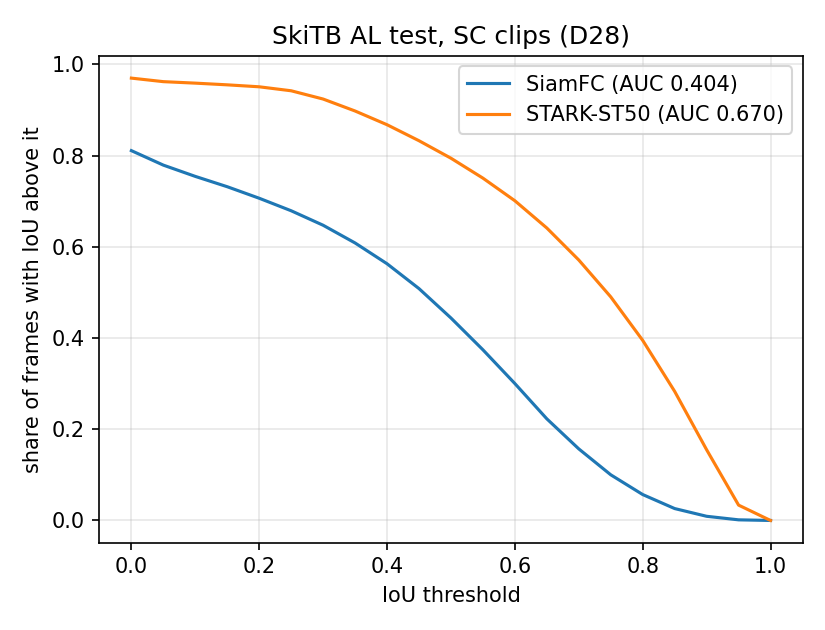
\includegraphics[width=0.6\linewidth]{figures/tracker_success_test.png}
  \caption{Extra experiment (Table~\ref{tab:extras}(a)): share of SkiTB test frames whose tracker box overlaps the
  ground truth above each IoU threshold, SiamFC vs off-the-shelf STARK-ST50 (471 clips). On val (75 clips): mean IoU
  0.363 vs 0.668 (+0.305 [0.254, 0.336]); E2 ski @0.1 under tracker crops 75.4 vs 88.0 (+12.6 [7.1, 20.2]), refined
  81.3 vs 90.9; replay box containment 0.943 vs 0.992. STARK's confidence threshold (0.33 on its probability) was
  chosen on val by the rule of Table~\ref{tab:choices}.}
  \label{fig:stark_success}
\end{figure}

\begin{figure}[h]
  \centering
  \includegraphics[width=\linewidth]{figures/pseudo_examples.png}
  \caption{Extra experiment (Table~\ref{tab:extras}(b)): pseudo-labels on six SkiTB training frames, one per race,
  picked at random with a fixed seed. Filled points and lines: joints kept by the filter, the student's training
  targets; hollow: the teacher's other body (blue) and ski (orange) points, dropped. Frames from
  SkiTB~\cite{dunnhofer2024tracking} (CC BY-NC 4.0).}
  \label{fig:pseudo}
\end{figure}

\end{document}
